\documentclass[border=3pt]{standalone}
\usepackage{tikz}
\usetikzlibrary{calc}
\begin{document}

\begin{minipage}{0.44\linewidth}
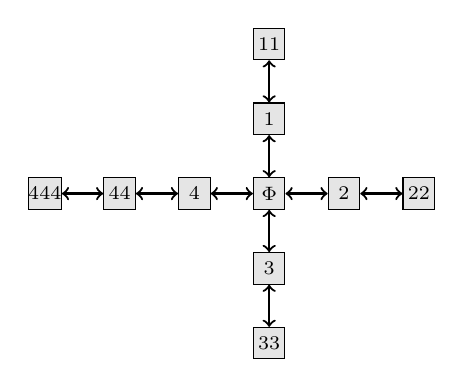
\begin{tikzpicture}[scale=0.95, state/.style={minimum width=4mm, minimum height=4mm, draw=black, fill=gray!20, inner sep=0pt, font=\scriptsize}]

\node[state] (0) at (0,0)  {$\Phi$};

\node[state] (1) at (0,1)  {$1$};
\node[state] (11) at (0,2)  {$11$};
%\node[state] (111) at (0,3)  {$111$};

\node[state] (2) at (1,0)  {$2$};
\node[state] (22) at (2,0)  {$22$};
%\node[state] (222) at (3,0)  {$222$};

\node[state] (3) at (0,-1)  {$3$};
\node[state] (33) at (0,-2)  {$33$};
%\node[state] (333) at (0,-3)  {$333$};

\node[state] (4) at (-1,0)  {$4$};
\node[state] (44) at (-2,0)  {$44$};
\node[state] (444) at (-3,0)  {$444$};

\foreach \x /\y in {444/44, 44/4, 4/0, 0/2, 2/22, 11/1, 1/0, 0/3, 3/33}
{\draw[<->, thick] (\x)--(\y);}
\end{tikzpicture}
\end{minipage}\hspace{10pt}
\begin{minipage}{0.55\linewidth}
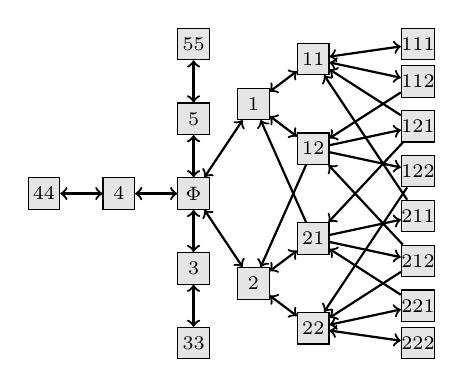
\begin{tikzpicture}[scale=0.95, state/.style={minimum width=4mm, minimum height=4mm, draw=black, fill=gray!20, inner sep=0pt, font=\scriptsize}]

\node[state] (0) at (0,0)  {$\Phi$};

\node[state] (5) at (0,1)  {$5$};
\node[state] (55) at (0,2)  {$55$};
%\node[state] (111) at (0,3)  {$111$};

\node[state] (3) at (0,-1)  {$3$};
\node[state] (33) at (0,-2)  {$33$};
%\node[state] (333) at (0,-3)  {$333$};

\node[state] (4) at (-1,0)  {$4$};
\node[state] (44) at (-2,0)  {$44$};
%\node[state] (444) at (-3,0)  {$444$};

\foreach \x /\y in {44/4, 4/0, 55/5, 5/0, 0/3, 3/33}
{\draw[<->, thick] (\x)--(\y);}

\node[state] (1) at (0.8,1.2)  {$1$};
\node[state] (2) at (0.8,-1.2)  {$2$};

\node[state] (11) at (1.6,1.8)  {$11$};
\node[state] (12) at (1.6,0.6)  {$12$};
\node[state] (21) at (1.6,-0.6)  {$21$};
\node[state] (22) at (1.6,-1.8)  {$22$};

\draw[<->, thick] (0)--(1);
\draw[<->, thick] (0)--(2);
\draw[<->, thick] (1)--(11);
\draw[<->, thick] (1)--(12);
\draw[->, thick] (21)--(1);
\draw[<->, thick] (2)--(21);
\draw[<->, thick] (2)--(22);
\draw[->, thick] (12)--(2);

\node[state] (111) at (3,2.0)  {$111$};
\node[state] (112) at (3,1.5)  {$112$};
\node[state] (121) at (3,0.9)  {$121$};
\node[state] (122) at (3,0.3)  {$122$};
\node[state] (211) at (3,-0.3)  {$211$};
\node[state] (212) at (3,-0.9)  {$212$};
\node[state] (221) at (3,-1.5)  {$221$};
\node[state] (222) at (3,-2)  {$222$};

\foreach \a/\b in {11/111, 11/112, 22/221, 22/222} {
  \draw[<->, thick] (\a)--(\b);
}

\foreach \a/\b in {11/121, 11/211, 12/112, 12/212, 21/121, 21/221, 22/122, 22/212} {
  \draw[<-, thick] (\a)--(\b);
}

\foreach \a/\b in {12/121, 12/122, 21/211, 21/212} {
  \draw[->, thick] (\a)--(\b);
}
\end{tikzpicture}
\end{minipage}


\end{document}
